\section{Comparison of the used methods of Kubernetes cluster deployment}
\label{6-comp}
\textit{In this chapter, several comparison criteria are used in order to compare the two chosen methods of a Kubernetes cluster deployment. The chapter ends with a summary deciding which method was better in relation to which comparison criterion.}
\\

Even though the two methods: using \textit{kops} and using \textit{eksctl}, help to deploy a Kubernetes cluster, they have some differences. For example: \textit{kops} works for many clouds (e.g. AWS, GCP), whereas \textit{eksctl} supports only AWS. Another difference is the default AMI. \textit{kops} chooses Debian Operating System, while \textit{eksctl} uses Amazon Linux 2. These AMIs are, however, only defaults, one can always choose another AMI. The mentioned differences can be known by skimming through the official documentation. On the contrary, this chapter is based on the empirical work.

\subsection{Production requirements which could not be satisfied}

There were nine production environment requirements which were supposed to be met by both tested methods. \textbf{All of them were met}. This means that both of the methods can be applied in production use cases. The table \ref{tab:comparison-prod-req} provides a brief explanation how each of the requirements was satisfied for each method.

Many requirements were handled in the same way for both methods. Subjectively, the hardest requirement to meet was: security, using \textit{eksctl}. There was a problem with finding a working \textit{YAML} configuration and also ensuring that cluster was healthy. \textbf{\textit{Eksctl} provides a more automated approach}. For example the \textit{AWS CloudWatch LogGroup}, needed for central logging, was automatically created when using \textit{eksctl}, but not when using \textit{kops}. Also, \textit{eksctl} provides the cluster which is already \textit{Highly Available}.

On the other hand, \textbf{\textit{kops} provides more flexibility}. The master node can be accessed with \textit{SSH} when using \textit{kops} and not when using \textit{eksctl}. When using \textit{kops}, it is possible to see all the kube-system namespaced pods, which is not the case with \textit{eksctl}. When using \textit{eksctl} no parameters of the control plane components can be set (to the best of the author's knowledge), with \textit{kops} it is possible.

\begin{table}[H]
\captionsetup{justification=centering}
\caption{\label{tab:comparison-prod-req}A comparison of how each production requirement was satisfied using the two methods: \textit{kops} and \textit{eksctl}}
\small
\begin{tabularx}{1\textwidth} {
  |>{\centering\arraybackslash}X
  | >{\centering\arraybackslash}X
  | >{\centering\arraybackslash}X |}
 \hline
  \textbf{Requirement} & \textbf{Using \textit{kops} method} & \textbf{Using \textit{eksctl} method} \\
 \hline
 A healthy cluster  & \multicolumn{2}{c|}{The same approach was used, \textit{Bats-core} was chosen as a test framework} \\
 \hline
 Automated operations  & \multicolumn{2}{c|}{The same approach was used, a \textit{Bash} file \textit{tasks} was used } \\
 \hline
 Central Monitoring & \multicolumn{2}{c|}{It was provided by AWS upfront, thanks to \textit{AWS CloudWatch} } \\
 \hline
 Central Logging  & Two \textit{Helm} charts were deployed & It was easy to configure with \textit{YAML} \\
 \hline
 Central Audit  & \multicolumn{2}{c|}{It was provided by AWS upfront, thanks to \textit{AWS CloudTrail} } \\
 \hline
 Backup  & \multicolumn{2}{c|}{The same approach was chosen, \textit{Velero} was used with an S3 bucket } \\
 \hline
 High Availability & It was easy to configure either with \textit{YAML} or CLI & It was provided by \textit{AWS EKS} upfront \\
 \hline
 Autoscaling  & \multicolumn{2}{c|}{The same approach was chosen, ClusterAutoscaler was deployed } \\
 \hline
 Security  & It was easy to set in \textit{YAML} & Finding a working \textit{YAML} configuration was more demanding \\
 \hline
\end{tabularx}
\end{table}





\subsection{Time of chosen Kubernetes cluster operations}
The next criterion used to compare the two deployment methods was time. \textbf{The time of several operations concerning Kubernetes cluster management was measured}. Each of the operation was performed several times and the mean value was used. Time was measured separately for \textbf{a minimal working cluster and for the full cluster}.

The minimal cluster here means such a cluster that is usable for end user and utilizes the default configuration (central monitoring, central audit, healthy cluster, automated operations are met). The production-grade cluster includes also the following requirements: HA, central logging and security. The about 5 min difference between creating a minimal and full cluster using \textit{eksctl} was caused by setting the security measures. The full cluster here does not include backup and autoscaling, because meeting these requirements is negligible in the terms of time and takes the same time for \textit{kops} and \textit{eksctl}.

Testing a cluster involves running the automated tests -- verifying that the cluster is healthy. It does not involve testing each of the production deployment requirements. Both the minimal and full clusters use \textit{t2.micro} for \textit{kops} and \textit{t2.small} for \textit{eksctl} for worker nodes. The time observed for the cluster operations is given in table \ref{tab:comparison-time} and in figure \ref{k8s-time}.

\begin{table}[H]
% force this caption to be put in one line
\captionsetup{justification=centering,margin=2cm,width=1.2\linewidth}
\caption{\label{tab:comparison-time}Time~needed~to~run~Kubernetes~management~operations~using~\textit{kops}~and~\textit{eksctl}}
\small
\begin{tabularx}{1\textwidth} {
  | >{\centering\arraybackslash}X
  | >{\centering\arraybackslash}X
  | >{\centering\arraybackslash}X |}
 \hline
  \textbf{Operation} & \textbf{Using \textit{kops} method} & \textbf{Using \textit{eksctl} method} \\
 \hline
 Create a minimal cluster  & 6 min 12 s & 19 min 26 s \\
 \hline
 Create a production-grade cluster  & 6 min 35 s & 25 min 40 s \\
 \hline
 Test a cluster  & 6 min 33 s & 6 min 40 s \\
 \hline
 Delete a cluster  & 2 min 23 s & 13 min 25 s \\
 \hline
\end{tabularx}
\end{table}

\begin{figure}[H]
    \centering
    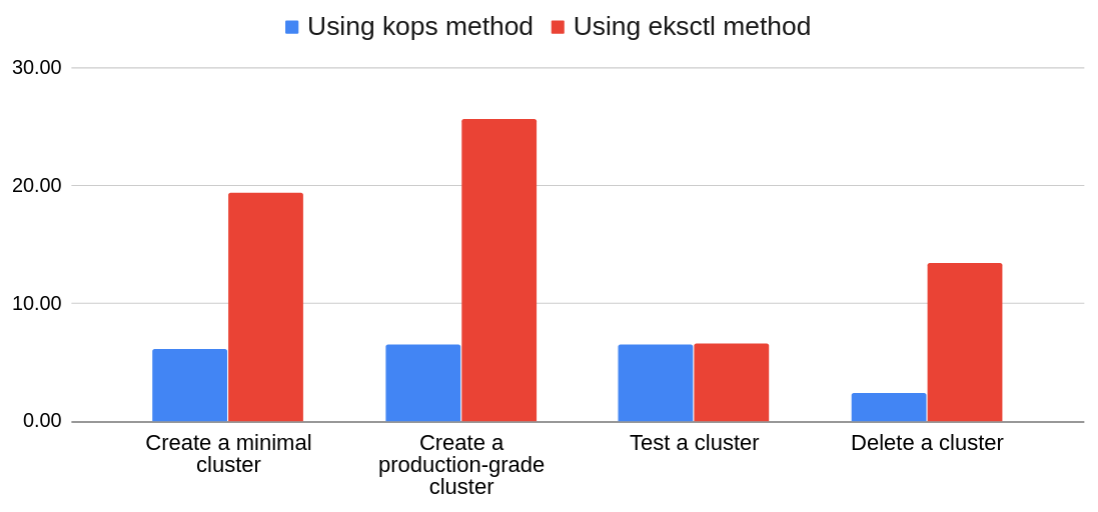
\includegraphics[width=15cm]{figures/k8s-time.png}
    % force this caption to be put in one line
    \captionsetup{justification=centering,margin=2cm,width=1.2\linewidth}
    \caption{Time needed to run Kubernetes management operations using \textit{kops} and \textit{eksctl}}
    \label{k8s-time}
\end{figure}


The files' names used to perform each cluster operation are demonstrated in table \ref{tab:comparison-which-file}. The files can be found in the public Git repository, presented in section \ref{5-sc}.
\begin{table}[H]
\captionsetup{justification=centering}
\caption{\label{tab:comparison-which-file}Files used to deploy minimal and full clusters using: \textit{kops} and \textit{eksctl}}
\small
\begin{tabularx}{1\textwidth} {
  | >{\centering\arraybackslash}X
  | >{\centering\arraybackslash}X
  | >{\centering\arraybackslash}X |}
 \hline
  \textbf{Which cluster} & \textbf{Using \textit{kops} method} & \textbf{Using \textit{eksctl} method} \\
 \hline
 A minimal cluster & \textit{src/kops/cluster-minimal.yaml} & \textit{src/eks/cluster-minimal.yaml} \\
 \hline
 A production cluster & \textit{src/kops/cluster.yaml} and central logging deployed & \textit{src/eks/cluster-minimal.yaml} \\
 \hline
\end{tabularx}
\end{table}

To summarize, it is clearly visible that operating a Kubernetes cluster is faster with \textit{kops}. The time of operations is an important criterion, because firstly, the faster it is, the faster one can get the feedback and experiment with the cluster. And secondly, longer creation and deletion times mean longer time of keeping AWS resources created, which in turn means that they cost more.

\subsection{Additional steps needed to create a Kubernetes cluster}
In order to deploy the clusters, many tools were needed. However, these tools were packaged inside a Docker image. Therefore, the development environment, provided by the Docker image was reliable and easily reproducible. It could be destroyed and recreated any time. But, apart from the development tools, there were also some prerequisites needed to be deployed for the production-grade clusters.

\textbf{When using \textit{kops}, one has to use and create an S3 bucket}. \textit{Kops} needs this bucket to store cluster configuration. Contrary to that, \textit{AWS EKS} does not need any additional AWS Resources created beforehands. However, this work attempted to deploy Kubernetes clusters in a production environment. In order to satisfy the backup requirement, \textit{Velero} was used. \textit{Velero} needs some location to store backups. In this work, a S3 bucket was used. Therefore \textbf{an S3 bucket was needed for both deployments}.

To summarize, both methods require the same steps to work in a production environment specified in this work, but the S3 bucket was used by choice and it could be replaced with some other storage solution.

\subsection{Minimal EC2 instance type needed for a Kubernetes worker node}
Various EC2 instances types cost various amount of money. Thus, it is preferable if one could use the cheapest possible instance type. It was proved, that \textbf{the smallest EC2 instance type, possible to be used in an AWS EKS cluster is \textit{t2.small}}. It was because of the hard limits set by AWS EKS for number of pods allowed for a particular EC2 instance type. The type \textit{t2.micro} allows for maximally 4 pods \cite{eks-hard-limits}. It was verified by experiment that \textit{eksctl} deploys 4 pods on a worker node, be design. Thus, there is no room left to deploy any application more. The type \textit{t2.small} allows for 11 pods.

Contrary to the AWS EKS cluster, there are no hardcoded limits for the number of pods when using \textit{kops}. \textbf{\textit{Kops} method allowed to use smaller instances of type: \textit{t2.micro}}. Using even smaller type (\textit{t2.nano}) resulted in the worker node being not accessible. There was no way to connect to the EC2 instance. The type \textit{t2.micro} was also used in some publicly available \textit{kops} tutorials, thus it was a proof that the practice matched the theory.

To summarize, \textbf{\textit{kops} clusters allows worker nodes of smaller and cheaper EC2 instance types}. The smallest working type for \textit{kops} is \textit{t2.micro}, whereas for \textit{eksctl}: \textit{t2.nano}.

\subsection{Easiness of configuration}

\textbf{With \textit{kops}, it was harder to generate the config file}. \textit{Kops}' documentation recommends that one should use \textit{kops create cluster} command instead of trying to generate it by hand. Using this command, one needs to create an S3 bucket first, the configuration file is put there and then, the object hosted on an S3 bucket can be exported to a local file. On the contrary, \textbf{with \textit{eksctl}, it was easier to generate the \textit{YAML} file and it was done by hand}.

On the other hand, \textbf{\textit{kops} allows for configuring the parameters of the control plane components, while \textit{eksctl} does not}. Another thing is, that \textbf{\textit{kops} allows using \textit{Golang templates}} \cite{online-kops-yaml-config-golang}. Thus, it is possible to use one template file and use it, for example, to deploy into two different environments: testing and production. However, since such templating solution was not possible with \textit{eksctl} (to the best knowledge of this work's author), in this work, template files with \textit{Bash} variables were used. It was easier to manage the template files for \textit{kops} and for \textit{eksctl} in the same way. This solution worked well and accomplished its purpose.

Considering the encountered problems, \textbf{there was an unexpected error, when creating the cluster with \textit{eksctl} and applying the security measure} to restrict the IP addresses which can access the API server. It was, subjectively, quite hard to find the working configuration and also it took long, because creating the not working cluster then, resulted in timeout after about 43 minutes. However, this problem was solved.

% * kops config change https://github.com/kubernetes/kops/blob/master/docs/changing_configuration.md
% * eksctl more magical and hidden config
% * eksctl: LogGroup on cloudWatch automatically created, little config, but not deleted on eksctl delete cluster
% * eks config iam - some in nodegroups, some under iam: ; not obvious what it concerns

\subsection{Meeting the automation requirement}

It is worth to summarize how it went to automate the cluster operations. Firstly, both \textbf{\textit{kops} and \textit{eksctl} automatically edited the kubeconfig file}. This was tremendously helpful, because immediately after cluster creation, one can access a cluster using \textit{kubectl} command.

Secondly, there was a difference concerning the moment in which the cluster creation commands return. \textbf{The \textit{kops} creation command returned immediately}. This means, that in order to automate the cluster creation to the extent that it can be run on a CI server, \textbf{some waiting mechanism was needed}. However, the waiting mechanism was easy to implement, because \textit{kops} provides the \textit{kops validate cluster} command. The command was run in a loop (with sleep in between each trial) and after is succeeded, the cluster was deemed created. On the other hand, \textbf{creating the cluster with \textit{eksctl} returned after all the AWS resources were created}.

Besides the aforementioned differences, \textbf{automating the operations was done in a very similar manner for both deployment methods}. Creating the configuration was harder with \textit{kops}, but this was a manual step and it does not need to be run on a CI server.

\subsection{Cost of chosen Kubernetes cluster operations}
In order to be aware of the cost generated by AWS resources needed to run the clusters, \textbf{an AWS tag was applied to all the AWS resources}. Thanks to such a solution, it was possible to use the \textbf{AWS Cost Explorer} to verify AWS resources cost. The particular tag applied was either \textit{deployment: eks-testing} or \textit{deployment: kops-testing}, depending on the deployment method used. In practice, no cluster was deployed with the label \textit{deployment: kops-production} or \textit{deployment: eks-production}, because in this work there was no difference between the testing and production environment. The intention of having 2 environments was to prove that all the configuration and operations can be automated for multiple environments and, so that in the future, it is possible to choose the environment. Chart taken from the AWS Cost Explorer website is presented in figure \ref{aws-cost-explorer}.

\begin{figure}[H]
    \centering
    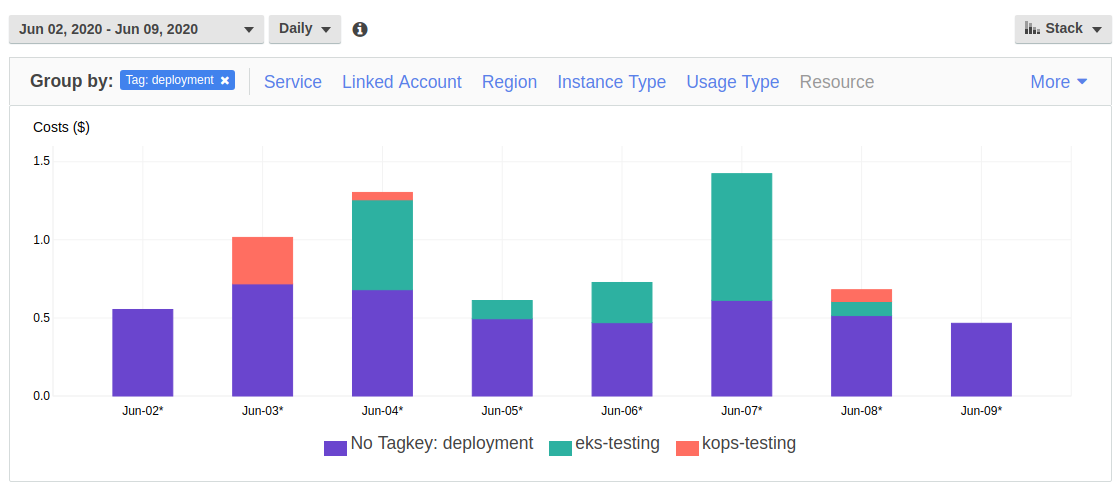
\includegraphics[width=15cm]{figures/aws-cost-explorer2.png}
    % force this caption to be put in one line
    \captionsetup{justification=centering,margin=2cm,width=1.2\linewidth}
    \caption{Cost report available on AWS Cost Explorer, grouped by the AWS tag: \textit{deployment}}
    \label{aws-cost-explorer}
\end{figure}

This chart should not be treated as a single source of truth, because firstly, the AWS tags were enabled later in the empirical work phase and secondly, experimenting with the clusters created with \textit{kops} took different amount of time and was performed different amount of times than experimenting with the clusters created with \textit{eksctl}. \textbf{The chart is just a way of showing an example how it is possible to monitor Kubernetes clusters cost}.

In order to be able to compare the cost of a cluster created with \textit{kops} and a cluster created with \textit{eksctl}, the following steps were taken.
\begin{enumerate}
\item A cluster was created with \textit{kops}, using the \textit{src/kops/cluster.yaml} file and central logging was deployed.
\item All the AWS resources decorated with the tag: \textit{deployment kops-testing} were listed with the following command: \textit{aws resourcegroupstaggingapi get-resources --tag-filters Key=deployment,Values=kops-testing}.
\item The \textit{kops} cluster was deleted.
\item A cluster was created with \textit{eksctl}, using the \textit{src/eks/cluster.yaml} file.
\item All the AWS resources decorated with the tag: \textit{deployment eks-testing} were listed with the following command: \textit{aws resourcegroupstaggingapi get-resources --tag-filters Key=deployment,Values=eks-testing}.
\item The \textit{AWS EKS} cluster was deleted.
\end{enumerate}

\textbf{This procedure resulted in two lists of all AWS resources, used by each Kubernetes deployment method}. Next, all the free AWS resources (\textit{VPC Subnets, Security Groups, Internet Gateway, Route Table}) were omitted. Overall, using \textit{eksctl}, the following AWS resources were used: \textit{1 Nat Gateway, 2 CloudFormation stacks, AWS EKS cluster, 2 EC2 instances} of type: \textit{t2.small} (used as worker nodes), an \textit{S3 bucket, 1 Load Balancer (ALB)} (to expose API server). For \textit{kops}, there was a bug and not all the AWS resources were tagged \cite{kops-issue-tags}. That bug should be fixed in the future releases of \textit{kops}, because there is already a PR merged on \textit{kops} \textit{Github.com} webiste \cite{kops-issue-tags-pr}. Despite this, it was possible to itemize the not free AWS resources used by \textit{kops}: 3 EC2 instances of type: \textit{t2.micro} (used as master nodes), 2 EC2 instances of type: \textit{t2.small} (used as worker nodes), 1 Load Balancer (ALB) (to expose API server), 6 EBS volumes (3 for \textit{etcd-main} and 3 for \textit{etcd-events}) of type gp2 and 20GB each, an S3 bucket. Whenever \textit{Elastic IPs} were used, they were omitted, because an attached Elastic IP does not cost anything.

Then, the cost for running a cluster for one month was computed. It is presented in tables \ref{tab:comparison-cost-eksctl} and \ref{tab:comparison-cost-kops}. Each of them lists the AWS resources used by one deployment method. \textbf{The last row of each table contains the total amount, in USD, of the monthly cost of the AWS resources}. The calculated cost does not include everything (e.g. transfer costs), but it should be enough to compare \textit{kops} to \textit{eksctl}. Many pricing information is given by Amazon per hour. 720 hours in a month was assumed. When it comes to \textit{CloudFormation} resources, there were 2 stacks used. The resources managed by the \textit{CloudFormation} stacks were received with the commands presented in listing \ref{lst:6-aws-cf}.
\begin{lstlisting}[basicstyle=\scriptsize,xleftmargin=0cm, label=lst:6-aws-cf,caption={AWS CLI commands used to list CloudFormation resources used by \textit{eksctl}},captionpos=b,language=Bash]
$ aws cloudformation list-stack-resources  --stack-name eksctl-eks-testing-nodegroup-ng-1
$ aws cloudformation list-stack-resources  --stack-name eksctl-eks-testing-cluster
\end{lstlisting}
The first stack managed 10 resources and the second stack - 34. The \textit{CloudFormation} pricing \cite{amazon-cf-pricing} depends on operations count. 10+34=44 creation operations and 10+34=44 deletion operations were assumed based on the information given. 88 operations total. The pricing website also informs that for operation durations above 30 seconds per operation, one will be charged \$0.00008 per second above the threshold. It cannot be assumed that all the resources took the same time to create, this was not measured. Thus, this cost is not included in the below calculations.

When it comes to the S3 cost, the storage cost is very cheap - \$0.023 for 1 GB \cite{s3-pricing}. The storage used by either \textit{kops} or \textit{eksctl} was for sure less than 1 GB, thus \$0.023 was assumed as monthly usage cost. Transfer costs were omitted.

\begin{table}[H]
% force this caption to be put in one line
\captionsetup{justification=centering,width=1.2\linewidth}
\caption{\label{tab:comparison-cost-eksctl}Expected cost of running a Kubernetes cluster created with \textit{eksctl} for one month}
\small
\begin{tabularx}{1\textwidth} {
  | >{\centering\arraybackslash}X
  | >{\centering\arraybackslash}X |}
 \hline
  \textbf{AWS Resource} & \textbf{Cost using \textit{eksctl} method} \\
 \hline
 1 Nat Gateway \cite{amazon-vpc-pricing} & 720 * \$0.048 = \$34.56 \\
 \hline
 Classic Load Balancer \cite{amazon-elb-pricing}  & 720 * \$0.028 = \$20.16 \\
 \hline
 2 CloudFormation stacks \cite{amazon-cf-pricing}  & 88 * \$0.0009 = \$ 0.0792 \\
 \hline
 AWS EKS cluster \cite{online-eks-pricing} & 720 * \$0.10 = \$ 72 \\
 \hline
 2 EC2 instances of type: \textit{t2.small} \cite{ec2-pricing}  & 2 * 720 * \$0.025 = \$36 \\
 \hline
 keeping files on S3 bucket \cite{s3-pricing}  & \$0.023 \\
 \hline
 \textbf{Total}  & \textbf{\$ 162.82} \\
 \hline
\end{tabularx}
\end{table}

\begin{table}[H]
% force this caption to be put in one line
\captionsetup{justification=centering,width=1.2\linewidth}
\caption{\label{tab:comparison-cost-kops}Expected cost of running a Kubernetes cluster created with \textit{kops} for one month}
\small
\begin{tabularx}{1\textwidth} {
  | >{\centering\arraybackslash}X
  | >{\centering\arraybackslash}X |}
 \hline
  \textbf{AWS Resource} & \textbf{Cost using \textit{kops} method} \\
 \hline
 5 EC2 instances of type: \textit{t2.micro} \cite{ec2-pricing} & 720 * \$0.0126 = \$ 9.072  \\
 \hline
 Classic Load Balancer \cite{amazon-elb-pricing}  & 720 * \$0.028 = \$20.16 \\
 \hline
 6 EBS volumes of type gp2 and 20GB each \cite{ebs-pricing} & 6 * 20 * \$0.11 = \$13.2 \\
 \hline
 keeping files on S3 bucket \cite{s3-pricing}  & \$0.023 \\
 \hline
 \textbf{Total}  & \textbf{\$42.46} \\
 \hline
\end{tabularx}
\end{table}

Based on the calculations provided above it costs \$ 162.82 to run a Kubernetes cluster created by \textit{eksctl} and \$42.46 to run a Kubernetes cluster created by \textit{kops}, on AWS, for a 30-day month. Some costs, e.g. data transfer, were not included.

% \subsection{Updating a running cluster}
% * how to change running cluster configuration
% * live upgrades


%* kops, s3 bucket for cluster store, versioning and encryption enabled,  The objects are encrypted using server-side encryption with either Amazon S3-managed keys (SSE-S3) or customer master keys (CMKs) stored in AWS Key Management Service (AWS KMS). https://docs.aws.amazon.com/AmazonS3/latest/dev/bucket-encryption.html; "There are no new charges for using default encryption for S3 buckets. Requests to configure the default encryption feature incur standard Amazon S3 request charges. " AES-256 (SSE-S3) https://docs.amazonaws.cn/en_us/AmazonS3/latest/user-guide/default-bucket-encryption.html; s3 data transfer pricing; maybe storage classes
%* load balancer for cluster as api endpoint and for each ing resources (kops) (avoiding LB: consider NodePort instead or also - would it work with curl http://api-endpoint -H 'my-ingress-url'?)
% * autoscaling from https://learnk8s.io/blog/kubernetes-chaos-engineering-lessons-learned to display the hostname of the current pod in a web page (so that we know if many pods are deployed?); kubectl scale then!
% "Service: A Kubernetes Service that identifies a set of Pods using label selectors. Unless mentioned otherwise, Services are assumed to have virtual IPs only routable within the cluster network." thus we use ingress https://kubernetes.io/docs/concepts/services-networking/ingress/ ; "Kubernetes Service with type: LoadBalancer -> Each Service spawns its own ELB, incurring extra cost." https://medium.com/@dmaas/amazon-eks-ingress-guide-8ec2ec940a70
% * what happens if we manually delete a iptables rule? kube-proxy will put it back after 10 to 30s - https://learnk8s.io/blog/kubernetes-chaos-engineering-lessons-learned

\subsection{Summary}

This was the main chapter of this work. It utilized the knowledge and experience gained throughout the previous, empirical chapters. The goal of this study was to compare two methods of a Kubernetes cluster deployment: using \textit{kops} and using \textit{eksctl}. In this chapter,  seven comparison criteria were applied. The criteria entailed: whether all the production environment requirements were met, time needed to operate a cluster, additional prerequisites, minimal EC2 instance types for worker nodes, easiness of configuration, meeting the automation requirement and cost of chosen Kubernetes cluster operations.

Some criteria are subjective, because one may enjoy having a wide choice of possible configuration to set, whereas another (or other use case) would prefer to create a cluster without a redundant hassle. Unquestionably: time and cost are the criteria helping us to decide objectively which method is better. Considering the two criteria, the winner is \textit{kops}. \textit{Kops} also provides more configuration options and can be applied on multiple clouds (not only AWS).

On the contrary, \textit{eksctl} provides an easier way to configure the cluster, because it is convenient to create a \textit{YAML} configuration file by hand. There are also no prerequisites needed before performing the deployment with \textit{eksctl}, unless one needs to satisfy the backup requirement. Then, some storage location (such as an S3 bucket) is needed. \textit{Kops} needs an S3 bucket to keep the cluster configuration. Besides, \textit{eksctl} provides a managed service (AWS EKS), thus the Kubernetes cluster administrator does not have to worry about managing the control plane components.

The last things that should be noted is that \textit{eksctl} is not the same as AWS EKS, even though \textit{eksctl} utilizes AWS EKS resource. Furthermore, all the results collected in this study may depend on the versions of \textit{kops}, \textit{eksctl} and maybe Kubernetes itself. This study used the particular versions of each tool and is based on the author's own experiments.
